% !TEX TS-program = pdflatex
% !TEX encoding = UTF-8 Unicode

% This is a simple template for a LaTeX document using the "article" class.
% See "book", "report", "letter" for other types of document.

\documentclass[11pt]{article} % use larger type; default would be 10pt

\usepackage[utf8]{inputenc} % set input encoding (not needed with XeLaTeX)

%%% Examples of Article customizations
% These packages are optional, depending whether you want the features they provide.
% See the LaTeX Companion or other references for full information.

%%% PAGE DIMENSIONS
\usepackage{geometry} % to change the page dimensions
\geometry{a4paper} % or letterpaper (US) or a5paper or....
% \geometry{margin=2in} % for example, change the margins to 2 inches all round
% \geometry{landscape} % set up the page for landscape
%   read geometry.pdf for detailed page layout information

\usepackage{graphicx} % support the \includegraphics command and options

% \usepackage[parfill]{parskip} % Activate to begin paragraphs with an empty line rather than an indent

%%% PACKAGES
\usepackage{booktabs} % for much better looking tables
\usepackage{array} % for better arrays (eg matrices) in maths
\usepackage{paralist} % very flexible & customisable lists (eg. enumerate/itemize, etc.)
\usepackage{verbatim} % adds environment for commenting out blocks of text & for better verbatim
\usepackage{subfig} % make it possible to include more than one captioned figure/table in a single float
% These packages are all incorporated in the memoir class to one degree or another...

%%% HEADERS & FOOTERS
\usepackage{fancyhdr} % This should be set AFTER setting up the page geometry
\pagestyle{fancy} % options: empty , plain , fancy
\renewcommand{\headrulewidth}{0pt} % customise the layout...
\lhead{}\chead{}\rhead{}
\lfoot{}\cfoot{\thepage}\rfoot{}

%%% SECTION TITLE APPEARANCE
\usepackage{sectsty}
\allsectionsfont{\sffamily\mdseries\upshape} % (See the fntguide.pdf for font help)
% (This matches ConTeXt defaults)

%%% ToC (table of contents) APPEARANCE
\usepackage[nottoc,notlof,notlot]{tocbibind} % Put the bibliography in the ToC
\usepackage[titles,subfigure]{tocloft} % Alter the style of the Table of Contents
\renewcommand{\cftsecfont}{\rmfamily\mdseries\upshape}
\renewcommand{\cftsecpagefont}{\rmfamily\mdseries\upshape} % No bold!

%%% END Article customizations

%%% The "real" document content comes below...

\title{Finding efficient harvest control rules for data limited fisheries management}
\author{
	Charles T T Edwards\textsuperscript{1} and Finlay Scott\textsuperscript{2}
	\\\textsuperscript{1,2}Imperial College London, UK\\\textsuperscript{2}CEFAS, UK
	}
\date{}

\begin{document}
\maketitle

\section{Introduction}

There is currently a growing debate surrounding the comparitive benefits of different harvest control rules for the managment of fisheries resources. In particular, whether model based control rules provide additional improvements to management in absolute terms. The contrarian view is that even when ample data are available for model fitting, model based control rules are too slow to allow extensive simulation testing. A more important point however, is that model based control rules are unable to fit to noisy data, so that as data paucity increases, performance declines. Importantly, performance may decline to levels below that which can be achieved with more simple empirical approaches. In other words, at low data levels, the more simple the harvest control rule, the better it is able to extract a signal from the data.

We test this idea using a simulation framework to quantify the relative performance of different harvest control rules and demonstrate that at low data levels, simple empirical control rules out perform more complex versions. At the same time our results highlight desirable qualities for control rules, namely the ability to maintain a consisitent level of performance across a wide range of data input levels.

\section{Theory}

Our aim is to find harvest control rules that perform well in data poor situations. This immediately raises two questions: how do we measure performance; and, how do we measure data poor? Only once measurements have been defined can examine the relation between them.

\subsection{Performance}
We take an information theoretic perspective on performancy, noting that the statistical efficiency of an estimation function $f$ measures the deviation of an estimated value $\hat{\theta}$ from the true value $\theta$:
\begin{equation}
e(f) = \frac{1/I(\theta)}{E[(\theta - \hat{\theta})^2]}
\end{equation}
where the numerator is the minimum variance that could be achieved (derived from the Fisher information $I()$) and the denominator is the actual variance obseved. Given that our harvest control rule is intended to estimate the catch $C$, from the above definition we obtain our measure of performance:
\begin{equation}
e(HCR) \propto \frac{1}{E[(C - \hat{C})^2]}
\label{eq:ehcr}
\end{equation}
Since $I(C)$ is undefined we note that this is a relative measure of efficiency only. However it has the intuitive property of measuring the variance of the estimated catch $\hat{C}$ around its \textit{real} value. This real value is defined as the catch which we would have set had we perfect knowledge of the status of the resource and its response to exploitation. 

\subsection{Data information}
Data \textit{quality} is ususally defined across more than one dimension. In this case we are concerned with an index of abundance only and consider the number of years and the observation error dimensions. Both of these dimensions contribute to the overall \textit{information} content of the data.

If $\varepsilon$ is the observation error residual, then the probability distribution of the mean residual is:
\begin{equation}
E[ln(\varepsilon)] \sim N\left(0,\sigma^2/n\right)
\end{equation}
From this relationship we define our measure of information content in the data, or conversly, data \textit{uncertainty}:
\begin{equation}
u(D) := \frac{\sigma}{\sqrt{n}}
\label{eq:datauncertainty}
\end{equation}

There may of course be other dimensions that should be considered. The availability of size frequency or age data for example could also provide additional information for the control. Further work of this nature will have to consider information measures that can accomodate these extra dimensions.

\section{Methods}

\subsection{Observation uncertainty}
We first obtained a relationship between the observation error surrounding a survey index and survey effort. This was achived by bootstrapping data from the ICES International Bottom Trawl Survey database, which is recorded at the level of individual tows. For each bootstrap sample, the number of tows used to estimate the mean index value could be changed to reflect different levels of survey effort. We varied the number of tows from 200 to 1200 (reflecting the approximate range in the database) and drew 1000 bootstrap samples for each effort value and for each year. The coefficient of variation across estimated mean values ($CV[\bar{I}]$) was then recorded. Finally we used non-linear least squares methods to fit a relationship between survey effort and the coefficient of variation. This fitted relationship is shown in Figure \ref{fig:obserror}.

\begin{figure}
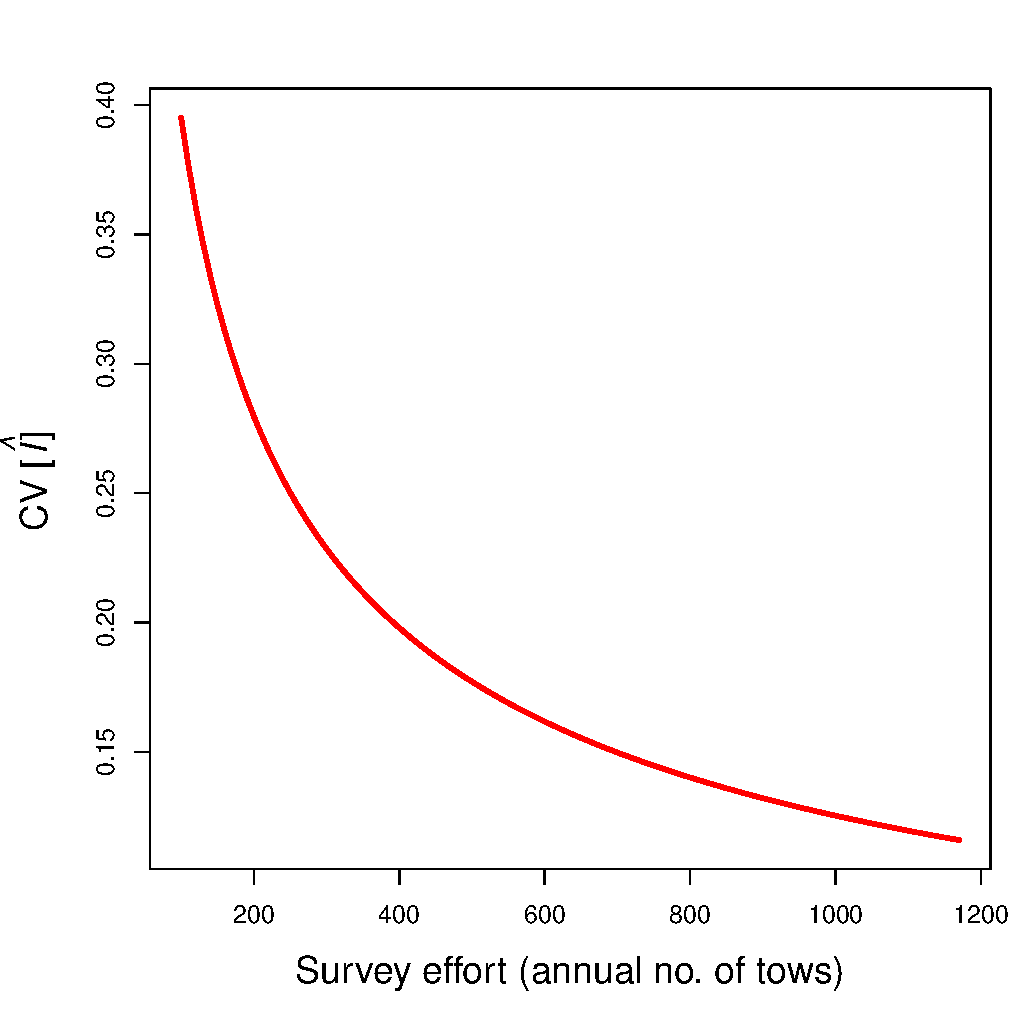
\includegraphics[width=0.9\textwidth]{../dat/obserror.pdf}
\caption{Fitted relationship between the coefficient of variation surrounding the survey abundance index and survey effort}
\label{fig:obserror}
\end{figure}

From the estimated relationship between observation error and $CV[\bar{I}]$, we can obtain our relationship between survey effort, the number of years of data and data uncertainty (Equation \ref{eq:datauncertainty}). This is shown in Figure \ref{fig:datauncertainty}.

\begin{figure}
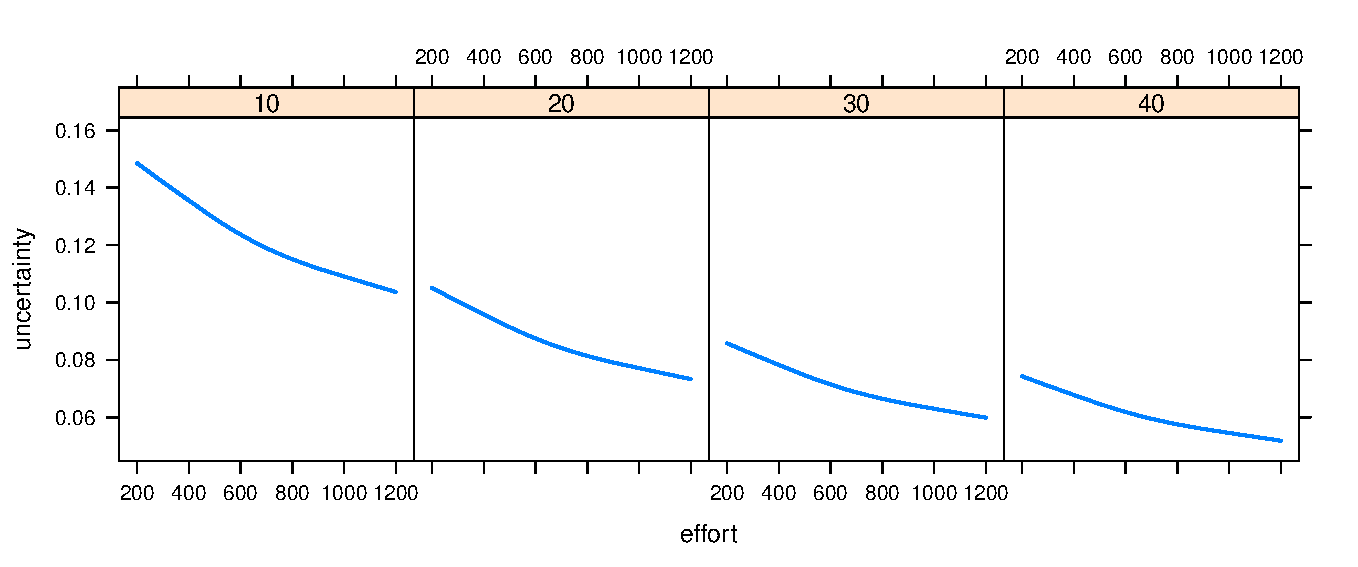
\includegraphics[width=1\textwidth]{../res/uncertainty.pdf}
\caption{Relationship between data uncertainty and survey effort for a range of $n$ values, corresponding to the number of years of data available}
\label{fig:datauncertainty}
\end{figure}

\subsection{Harvest control rule}

A large number of index based harvest control rules are available in the literature. Those of an empirical nature usually require a degree of \textit{tuning} to optimise the probability that the resource reaches target biomass or catch levels within a specified time frame. Tuning is tangental to the problem being addressed here and we therefore adopt a control rule for which it is implicit. This requires us to assume some additional knowledge, namely known target levels for the exploitable biomass and catch ($B^{TAR}$ and $C^{TAR}$ respectively). These reference points were set externally to levels associated with the Maximum Sustainable Yield (MSY), which would normally be estimated during stock assessment. To ensure equivalence, the same reference points were used by the model based control rules.

The catch algorithm takes the form:
\begin{equation}
C_{y+1} = \frac{G(B_{y+1})C^{TAR}}{G(B^{TAR})}
\label{eq:hcr}
\end{equation}
Model based control rules are able to predict the biomass, and in this case therefore the function $G(B) = B$. Empirical control rules however are only able to predict index values. Noting that the target biomass $B^{TAR}$ is equivalent to a target index value, since $I^{TAR} = qB^{TAR}$, we are able to define $G(B) = I$ for the empirical control rules assuming the catchability $q$ is known. This additional assumption allows us to maintain direct comparability of performance across model based and empirical approaches.

We are interested in the perfomance of different methods of predicting $B_{y+1}$ or (equivalently) $I_{y+1}$. Four different approaches were compared here:
\begin{itemize}
\item Moving average
\item Linear regression
\item Smoothed index (Double exponential smoothing)
\item Model-based (Stock reduction analysis estimating $B_0$, $q$ and $\sigma$)
\end{itemize}


\subsection{Simulations}

An operating model was developed by first obtaining life-history parameters from FLH, and then using these to paramaterise an age structured production model. The population was assumed to be fully selected. We applied an historic time series of fishing mortalities to initialise the current population biomass and then projected forward for a period of 60 years with the control rule applied. Information provided to the control rule was varied by changing the number of years of data available (as a sliding window of 5 to 40 years), and the number of survey tows per year (from 200 to 1200). Stochasticity was introduced via the recruiment residuals and observation error. For each value of observation error ($\sigma$) and number of years ($n$), we performed 20 iterations of the control rule projection, recording the performance measure (Equation \ref{eq:ehcr}) for each.

Convergence of the model based control rule can never be ensured during simulation testing of performance. However we took appropriate measures to promote convergence. First, we initialised the optimisation at the true value; second we only allowed a small degree of residual variation around the stock recruitment relationship.

\section{Results}

Illustrative results are shown in Figure \ref{fig:ires}, which indicates how greater data uncertainty leads to higher variation in the predicted index value. This variation is quantified by the performance measure and full simulation results are shown in Figure \ref{fig:fres}. We note that good performance implies that the target catch and biomass (or index) values are closer to being met, since the estimated catch will be closer to that which would have been taken assuming perfect knowledge of the resource. 

\begin{figure}
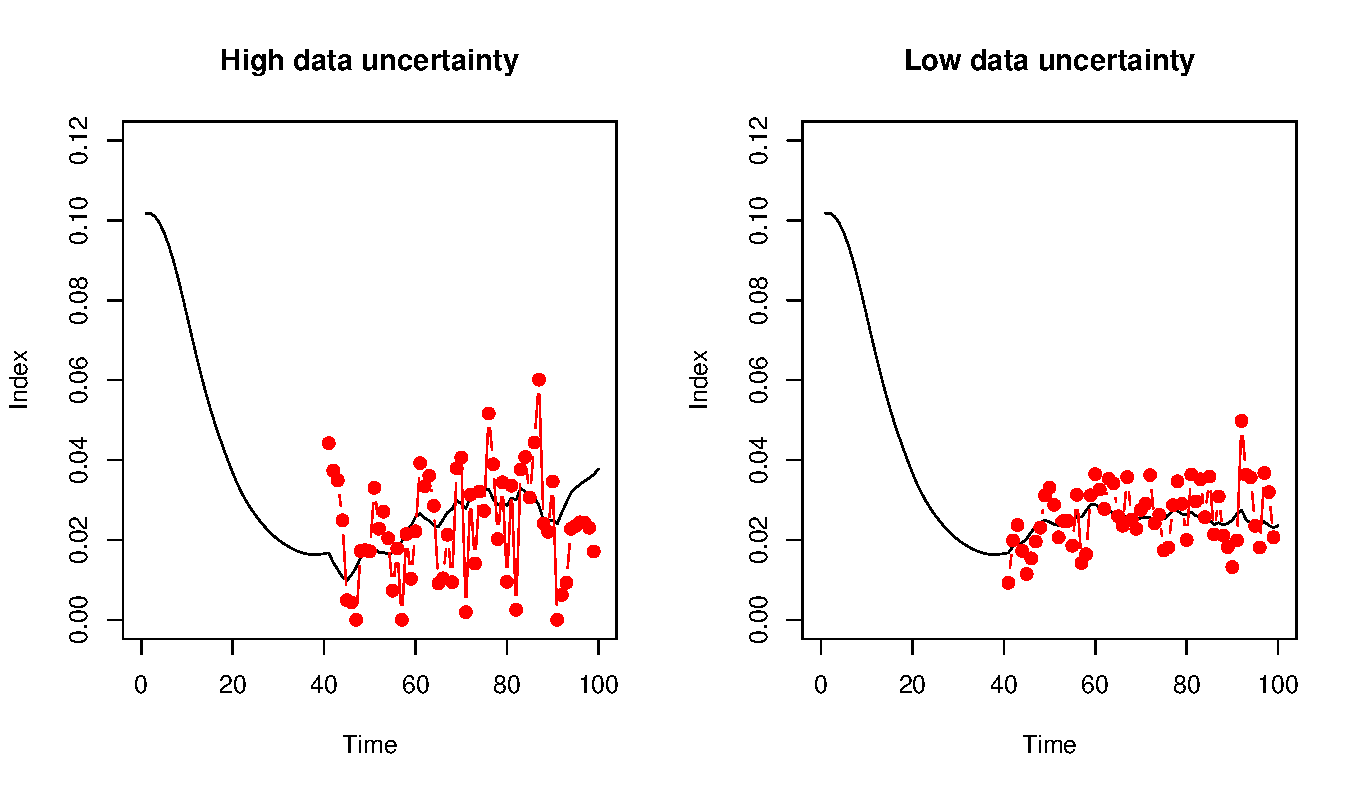
\includegraphics[width=0.9\textwidth]{../res/uncertainty_index.pdf}
\caption{Illustrative results: Predicted index values are shown for each year under high and low data uncertainty scenarios. The true index value is shown as a solid line. The harvest control rule used a smoothed index value to obtain the catch for each year and was applied from year 41 onwards.}
\label{fig:ires}
\end{figure}

\begin{figure}
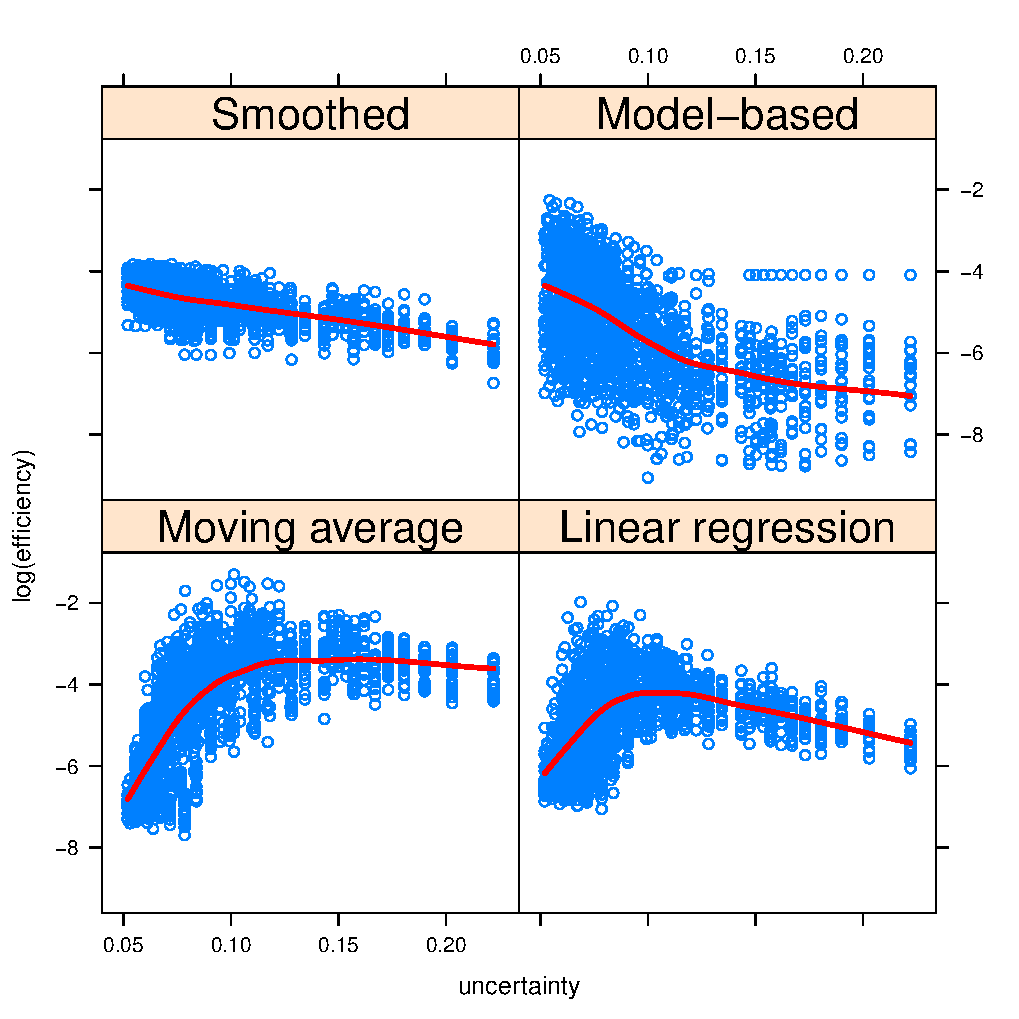
\includegraphics[width=0.6\textwidth]{../res/hcr_all_plot.pdf}
\caption{Performance: Scatter plots of performance against data uncertainty for the four harvest control rules.}
\label{fig:fres}
\end{figure}

\section{Conclusions}

We are primarily interested in the performance of model based and empirical control rules under data-poor conditions when data uncertainty is high. It is clear that in this situation the model based control rule is out-performed by the emprirical control rules. This implies that the more simple empirical control rules are able to make better use of the available data to estimate appropriate catch levels. In other words, they are more efficient. 

In any managment situation it is difficult to assess data paucity, which is a subjective measure, and whether the data contains enough information to support a model based control rule. A precautionary approach therefore would be to apply a control rule that is able to maintain performance accross a range of uncertainty levels (i.e. that is robust to increased uncertainty in the input data). Thus, even though the model based control rule performs well when the data quality is good, this is not sufficient grounds for promoting its use. 

The discussion surrounding a need robust control rules highlights desirable properties that could be used to inform their design. As already indicated, control rules that have a declining performance at high data uncertainty are not desirable. However it is also true that control rules that have a declining peformance at low data uncertainty are also not desirable. This property is illustrated by the moving average and regression based control rules, which become less sensitive as more information is supplied (primarily due to an increased number of years which leads to the unwarranted influence of historic index values). 

The smoothed control rule appears to have desirable properties, since performance is consistently maintained at high and low levels of data uncertainty. Such generic insights are useful for the design of management stratgies where data paucity cannot be quantified, particularly if stock dynamics are poorly defined, preventing full simulation testing of the control rule.


\end{document}


% TO DO
% - derive measure of data information that can accomodate more dimensions e.g entropy
% - integrate over a range of initial conditions e.g. rebuild; fishing down
% - try other control rules e.g. simple model based B = B + Rhat - C
% - can we bring it to life with a 'real' example e.g. NS cod, plaice?



